\documentclass[12pt, letterpaper, twoside]{article}
% ========= Preamble ========
\usepackage[utf8]{inputenc}
%% Packages: 
%%% for displaying images:
\usepackage{graphicx}
%%%% settings for graphicx:
%%%%% path
\graphicspath{img/}
 
\title{First document}
\author{Andrzej Zahorski \thanks{thanks the Internet}}


% ======== /Preamble =========
\begin{document}
 
\maketitle
 
We have now added a title, author and date to our first \LaTeX{} document!
\subsection{Bold, italics, underlining}
\begin{itemize}
\item \textbf{Texting to best friend (bold is textbf) xD - bold} 
\item \textit{viva la pizza di cardinale - italics} 
\item \underline{underlined text here - underline} 
\end{itemize}
% SUBSECTION
\subsection{Different faces of \emph{emphasizing}:} 
\begin{itemize}
    \item \emph{inside normal text emphasized text is italicized}
    \item \textit{\emph{result of emphasis in italicized text - both things are canceling each other out}}
    \item \textbf{\emph{this is the effect of emphasis inside bold text = bold + italics}}
\end{itemize}

% SUB
\subsection{}
\begin{itemize}
    \renewcommand\labelitemi{--}
    \item \LaTeX{} does not render images by itself, we need \textbf{graphicx} package
    \item  we set path for it in Preamble
    \item then we use \textit{includegraphics}
    \end{itemize}

\includegraphics[scale=0.5]{img/cat}
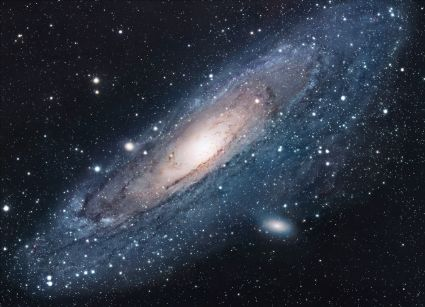
\includegraphics[width=\textwidth]{universe}


\end{document}